\section{Light Curves}


\begin{frame}{AB magnitudes at 40Mpc for DD2\_q1.67 and BLh\_q1.43}

\begin{minipage}[t]{0.48\textwidth}
\vspace{0pt}
        \begin{figure}
                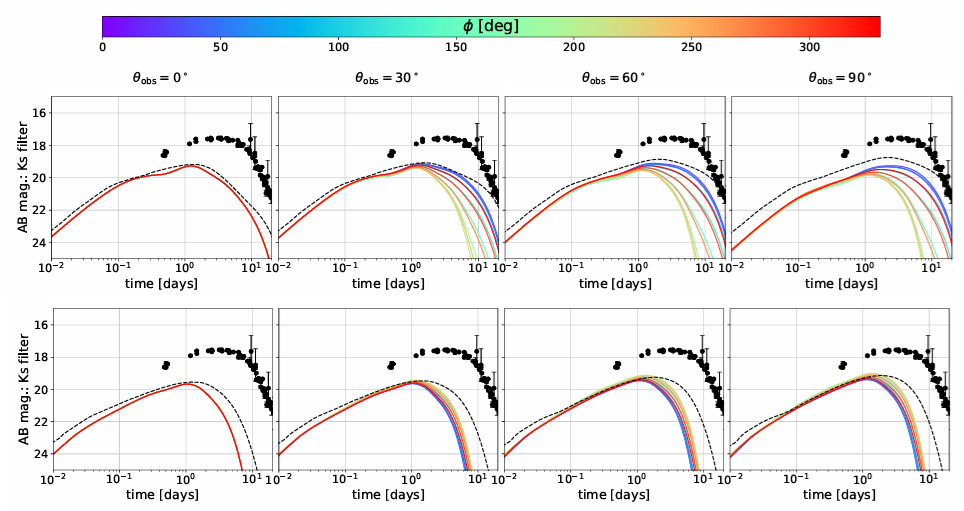
\includegraphics[width=\linewidth]{../fig/model_comparison/ABmagnitudes_DD2A_BLH.png}

        \end{figure}

\end{minipage}
\hfill
\begin{minipage}[t]{0.48\textwidth}
\vspace{0pt}
\begin{tcolorbox}[
    colback=white,
    colframe=blue,
    colbacktitle=blue!50!black!50,
    title=Discussion,
    fonttitle=\bfseries,
    rounded corners,
    boxrule=1pt,
    left=2mm, right=2mm, top=1mm, bottom=1mm
]
\begin{itemize}
   \scriptsize 
    \item Comparison with 2D simulations
    \item Comparison with AT2017gfo data 
    \item Extra $\phi$-dependence does not bridge the gap
    \item Can actually work the other way around
    \item Bigger difference in the Ks filter
    \item Effect of the "lack" of a lanthanide curtain at $\theta\sim200^{o}$  for DD2\_q1.67 
\end{itemize}
\end{tcolorbox}
\end{minipage}

\end{frame}
